\subsection{Comparison for Px}
\label{subsec:comparison}

Now, it can be interesting to compare the results obtained with the different linearization/approximation described in the previous sections.
For simplicity, we will perform this type of error analysis only for the force $P_x = f(\vec{u})$, but conceptually it would be the same for the force $P_y = f(\vec{u})$.

Since the following doesn't want to be a formal error analysis, we will not use any formal error measure, but we will simply plot the difference between the approximated / linearized solutions and the exact one, that is:

\begin{equation}
    z(u,v) = \text{Error}[P_x(u,v)] = P_{x,approximated/linearized}(u,v) - P_{x,exact}(u,v)
\end{equation}

In this way, the error analysis can be performed graphically, by plotting a 3D surface of the error in the space $(u,v,z)$.

Moreover, since all our linearized / approximated solutions were obtained in the neighborhood of the point $\vec{u} = \vec{0}$ (because of the hypothesis of small displacements), we will limit our plot to a domain of $(u,v) \in [-0.01, 0.01] \times [-0.01, 0.01]$
\footnote{At this point the choice of the domain dimension has been done per intuition. A post analysis with the numerical result at hand, would show that this domain is far too large with respect to the solutions effective domain $(\text{Factor}=10^2)$.}.

\begin{figure}[H]
    \centering
    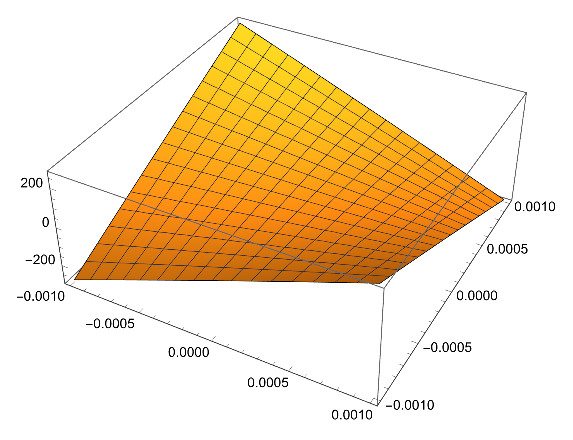
\includegraphics[width=.5\textwidth]{./pdf/error_taylor_order_1}
    \caption{Error analysis for a Taylor series of order 1}
    \label{fig:error_taylor_order_1}
\end{figure}

\begin{figure}[H]
    \centering
    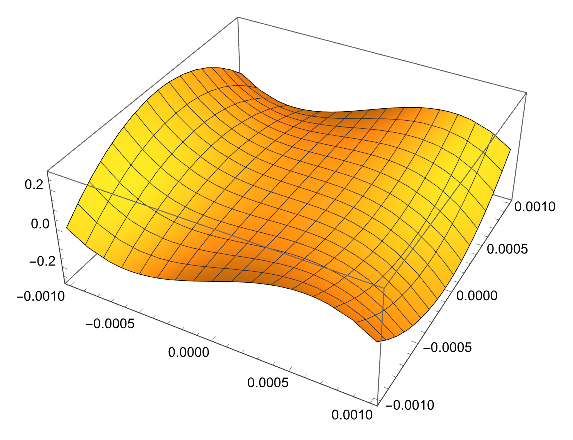
\includegraphics[width=.5\textwidth]{./pdf/error_taylor_order_2}
    \caption{Error analysis for a Taylor series of order 2}
    \label{fig:error_taylor_order_2}
\end{figure}

\begin{figure}[H]
    \centering
    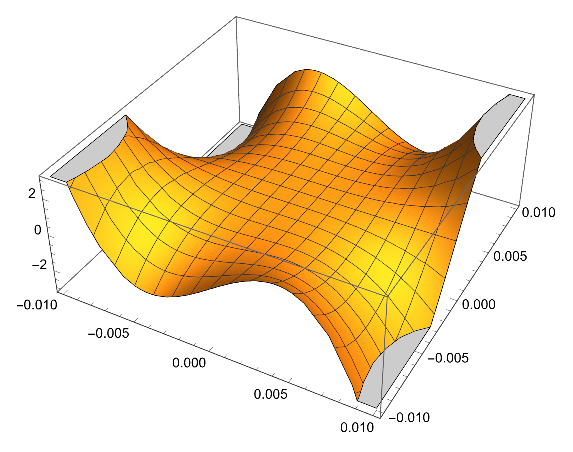
\includegraphics[width=.5\textwidth]{./pdf/error_taylor_order_3}
    \caption{Error analysis for a Taylor series of order 3}
    \label{fig:error_taylor_order_3}
\end{figure}

% \begin{figure}[H]
%     \centering
%     \includegraphics[width=.5\textwidth]{./pdf/error_taylor_order_4}
%     \caption{Error analysis for a Taylor series of order 4}
%     \label{fig:error_taylor_order_4}
% \end{figure}

\begin{figure}[H]
    \centering
    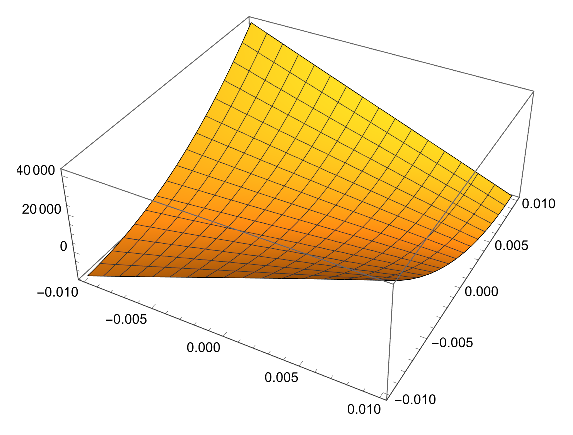
\includegraphics[width=.5\textwidth]{./pdf/error_approximated_soft}
    \caption{Error analysis for approximated (soft) solution}
    \label{fig:error_approximated_soft}
\end{figure}

\begin{figure}[H]
    \centering
    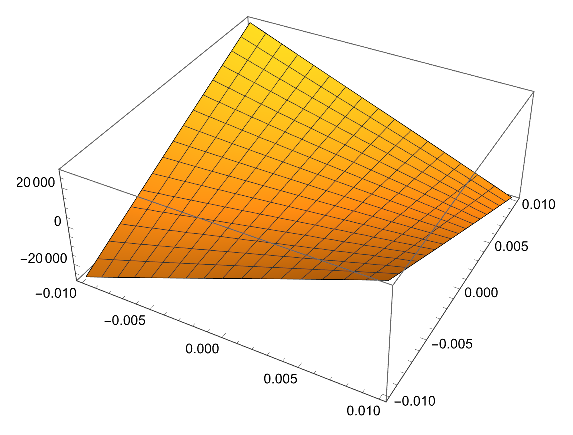
\includegraphics[width=.5\textwidth]{./pdf/error_approximated_hard}
    \caption{Error analysis for approximated (hard) solution}
    \label{fig:error_approximated_hard}
\end{figure}

As we can see, in the neighborhood of point $\vec{u} = \vec{0}$, the error is negligible for every linearization and/or approximations.

However, as we move away from the point $\vec{u} = \vec{0}$, the error increases.
In particular, we can see that the error introduced by the linearization decreases as we increase the order of the Taylor series expansion.